% =====================================================================
%  Manuscript for Biomedical Signal Processing and Control (Elsevier)
%  Official elsarticle class (TeX Live elsarticle.cls), preprint, 12pt,
%  numbered references (elsarticle-num.bst). Every number traces to reports/.
% =====================================================================
\documentclass[preprint,12pt]{elsarticle}
\usepackage{amsmath,amssymb}
\usepackage{graphicx}
\usepackage{booktabs}
\usepackage{multirow}
\usepackage[T1]{fontenc}
\usepackage{lmodern}
\usepackage{textcomp}
\usepackage[hidelinks]{hyperref}
\usepackage{lineno}

\journal{Biomedical Signal Processing and Control}

\begin{document}

\begin{frontmatter}

\title{Eight-bit quantization of tiny wrist-inertial networks for Parkinson's disease detection: a pre-specified empirical study with microcontroller validation}

\author[hcmute]{Quang-Tuyen Lai}
\ead{2612108@student.hcmute.edu.vn}

\author[hcmute]{Ba-Viet Ngo\corref{cor1}}
\ead{vietnb@hcmute.edu.vn}
\cortext[cor1]{Corresponding author.}

\affiliation[hcmute]{organization={Faculty of Electrical and Electronics Engineering, Ho Chi Minh City University of Technology and Engineering},
            addressline={1 Vo Van Ngan Street, Thu Duc},
            city={Ho Chi Minh City},
            postcode={700000},
            country={Vietnam}}

\begin{abstract}
Wrist-worn inertial sensors could support Parkinson's disease screening if the classifier runs on the wearable itself, which usually requires eight-bit integer arithmetic. Under an analysis plan fixed in advance, we tested whether quantization preserves the accuracy of a depthwise-separable temporal convolutional network with 22.7k parameters on a public smartwatch dataset of 469 participants. We used participant-level nested cross-validation, three training seeds and 14 simulated device shifts. In the pre-specified pooled analysis, post-training quantization was not non-inferior to full precision in any seed (area under the receiver operating characteristic curve lower by 0.033 to 0.064), quantization did not add loss under shift, and quantization-aware training with sensor randomization outperformed post-training quantization in two of three seeds. Exploratory within-fold analyses showed that the post-training loss averaged 0.066, reached 0.219 in one fold, was not removed by more calibration data and vanished when activations were kept at 16 bits. Quantization-aware training showed no detectable loss, and sensor randomization gave no consistent benefit. Pooling predictions across temperature-scaled folds understated the full-precision area under the curve by more than 0.1. On an ESP32-S3 microcontroller, a streaming pipeline gave bit-exact outputs in 12.6~ms per 2-s step with 39.4~kB of memory, provided the network was trained with the device's causal filter. A feature-based random forest was more accurate and also ran on the device. Eight-bit activations, not weights, made post-training quantization of this network unreliable; quantized wearable models should be validated per fold, across seeds and with on-device preprocessing.
\end{abstract}

\begin{keyword}
Parkinson's disease \sep Wearable inertial sensors \sep Quantization \sep Tiny machine learning \sep Microcontroller \sep Domain shift \sep Pre-specified analysis
\end{keyword}

\end{frontmatter}

\linenumbers

% =====================================================================
\section{Introduction}
\label{sec:intro}
Parkinson's disease (PD) is the fastest-growing neurological disorder; the number of affected people more than doubled between 1990 and 2016~\cite{GBD2018PD,Dorsey2018}. Diagnosis still rests on clinical examination and rating scales such as the MDS-UPDRS~\cite{Goetz2008,Postuma2015}. Wrist-worn inertial sensors offer a cheap, objective complement. Smartwatches can capture tremor, bradykinesia and dyskinesia in the clinic and at home~\cite{Rovini2017,Sigcha2023rev,Powers2021,Lipsmeier2018}, and public datasets now allow fair comparison of methods~\cite{Varghese2024,Bot2016,Monipar2023}.

For screening at scale, the model should run on the wearable itself. On-device inference keeps raw signals private, works without a network connection and saves the energy spent on radio transmission. Microcontrollers, however, have a few hundred kilobytes of memory and favour eight-bit integer arithmetic~\cite{David2021,Lin2020,Banbury2021,Ray2022}. Models must therefore be small and quantized~\cite{Jacob2018,Krishnamoorthi2018,Nagel2021}.

Two questions are rarely asked together. First, does a tiny PD model keep its accuracy after quantization? In wearable heartbeat classification, post-training quantization cost several points of accuracy~\cite{Nikandish2026}; in embedded electrocardiogram classification, it shifted output scores enough to break a calibration derived from the full-precision model~\cite{ElAllam2026}. Existing tiny PD systems report accuracy on self-collected data only~\cite{Parikh2026}. Second, does the model keep its accuracy when the device changes? Accelerometers of different brands produce non-equivalent raw signals~\cite{CoyleAsbil2026}, sensor heterogeneity degrades activity recognition~\cite{Stisen2015}, and domain-adaptation methods for wearables need data from the target domain~\cite{Zhu2025,Zheng2026}. Studies on the public PADS dataset report results on that dataset alone, with full-precision models~\cite{Varghese2024,Zannat2026}. Finally, splitting by recording instead of by participant inflates accuracy~\cite{Saeb2017,Kapoor2023}, and models that look strong internally often fail on external data~\cite{Zech2018,Kelly2019}.

We found no study that tests a quantized PD model under device shift with participant-level evaluation and on-device verification. This paper reports such a study as an empirical evaluation, not as a new architecture. We ask three research questions (RQs). RQ1: how do tiny networks compare with feature models under a leakage-free, participant-level protocol? RQ2: how much accuracy does eight-bit quantization cost, in distribution and under device shift? RQ3: can the training procedure remove this cost without extra on-device resources? The main findings are:
\begin{itemize}
  \item In a pre-specified, three-seed analysis with 14 simulated device shifts, post-training quantization of a depthwise-separable network was not non-inferior to full precision; its loss did not grow under shift.
  \item Exploratory analyses located the loss in 8-bit activations, showed that quantization-aware training avoided it at no device cost, and found no consistent benefit from sensor randomization.
  \item Pooling cross-validated predictions across temperature-scaled folds distorted the area under the curve; within-fold metrics were needed to interpret the planned tests.
  \item On an ESP32-S3 microcontroller, inference was bit-exact and took 12.6~ms per 2-s streaming step, but only a network trained with the device's causal filter kept its accuracy.
\end{itemize}

% =====================================================================
\section{Related work}
\label{sec:related}
\emph{Wearable PD assessment.} Reviews describe a large body of work on inertial sensing for PD diagnosis and monitoring, most of it with single-site data~\cite{Rovini2017,Sigcha2023rev}. The PADS dataset provides 469 participants with two smartwatches and 11 neurologist-designed tasks; its authors reported nested cross-validation for PD versus controls and versus differential diagnoses~\cite{Varghese2024}. Later work on PADS reported accuracies above 90\% with a label-efficient bilateral attention network and 124.5~ms per window on a Raspberry Pi~4~\cite{Zannat2026}; the abstract does not describe the split. A frequency-aware adversarial network was also evaluated on PADS~\cite{Zhao2025MFAM}. Multiple-instance learning has been used to aggregate window evidence into person-level tremor labels in free-living data~\cite{Papadopoulos2023,Ilse2018}, and tremor has been detected in the wild with wrist accelerometers~\cite{SanSegundo2020}. Smartwatch tremor and bradykinesia assessment was also studied on the Monipar cohort~\cite{Sigcha2021,Monipar2023}. Shoe-embedded inertial and pressure sensors separated PD from normal pressure hydrocephalus in 23 patients under nested cross-validation, with an area under the curve of $0.74 \pm 0.39$, which illustrates how variable small-cohort estimates are~\cite{Magni2026}.

\emph{Device shift and evaluation.} Differences in sampling rate, timing and sensor quality between devices reduce recognition accuracy~\cite{Stisen2015}. On a shaker table, raw accelerations from different brands differed significantly at higher frequencies, and low-pass filtering improved their equivalence~\cite{CoyleAsbil2026}. Cross-domain activity recognition has been addressed with domain adaptation and fused attention~\cite{Zhu2025} and with few-shot adaptation across positions, users and datasets~\cite{Zheng2026}; both need some target data. Augmenting wearable data with rotations and noise improved PD motor-state detection~\cite{Um2017}, and randomizing simulated conditions can transfer models without target data~\cite{Tobin2017}. Our sensor randomization follows this idea.

\emph{Tiny models for biomedical signals.} Depthwise-separable and temporal convolutional networks reduce computation for sequence data~\cite{Howard2017,Bai2018}. Integer-only inference and quantization-aware training are standard for deployment~\cite{Jacob2018,Krishnamoorthi2018,Nagel2021}. Federated TinyML has been proposed for micro\-con\-trol\-ler-based medical devices~\cite{Ibrar2026}, and hybrid multi-timescale networks decoded surface electromyography on STM32 microcontrollers, with complexity estimates checked against measured latency~\cite{Ortone2026}. A compressed Bi-LSTM showed that post-training quantization can reduce heartbeat-classification accuracy~\cite{Nikandish2026}. For electrocardiogram classification on an ESP32-S3, conformal calibration derived from full precision under-covered after INT8 quantization, and recalibrating on the INT8 outputs restored coverage~\cite{ElAllam2026}. A quantized glove model for PD ran on an Arduino board but was tested only on self-collected data~\cite{Parikh2026}. Table~\ref{tab:related} summarizes the differences.

\begin{table}[!t]
\caption{Comparison with prior work.}
\label{tab:related}
\centering\small\setlength{\tabcolsep}{4pt}
\resizebox{\textwidth}{!}{%
\begin{tabular}{@{}lccccc@{}}
\toprule
Study & Data & Participant split & External & INT8 & MCU \\
\midrule
Varghese et al.~\cite{Varghese2024} & PADS & \checkmark & -- & -- & -- \\
Zannat~\cite{Zannat2026} & PADS & n.r. & -- & -- & -- \\
Papadopoulos and Delopoulos~\cite{Papadopoulos2023} & Free-living & \checkmark & -- & -- & -- \\
Parikh et al.~\cite{Parikh2026} & Own glove (PD) & \checkmark & -- & \checkmark & \checkmark \\
Nikandish et al.~\cite{Nikandish2026} & ECG & n.a. & -- & \checkmark & n.r. \\
El Allam and Hamlich~\cite{ElAllam2026} & ECG & \checkmark & (\checkmark)$^{b}$ & \checkmark & \checkmark \\
This work & PADS + Monipar & \checkmark & (\checkmark)$^{a}$ & \checkmark & \checkmark \\
\bottomrule
\end{tabular}}

\vspace{2pt}\parbox{\linewidth}{\footnotesize External: second cohort. MCU: run on a microcontroller. n.r.: not reported. n.a.: not applicable. $^{a}$Zero-shot, descriptive only (7 controls). $^{b}$Second dataset evaluated with its own calibration.}
\end{table}

% =====================================================================
\section{Materials and methods}
\label{sec:methods}
\subsection{Datasets}
The Parkinson's Disease Smartwatch dataset (PADS)~\cite{Varghese2024,PADSdata} was recorded at a movement-disorder outpatient clinic with two Apple Watch Series~4 devices, one on each wrist, while participants were seated. Each participant performed 11 interactive movement steps of 10 to 20~s designed by neurologists (resting, postural and kinetic tasks). Tri-axial acceleration (g) and angular velocity (rad/s) were sampled at 100~Hz; the released acceleration has gravity removed. The cohort comprises 469 participants: PD (276), healthy controls (HC, 79) and differential diagnoses (DD, 114: other movement disorders 60, essential tremor 28, atypical parkinsonism 15, multiple sclerosis 11). Diagnoses were confirmed by board-certified neurologists. PADS was used for nested cross-validation.

Monipar~\cite{Monipar2023,MoniparData} contains 28 participants (21 PD, of whom 6 were supervised and 15 recorded at home; 7 HC) with 174 trials. A single smartwatch model (TicWatch S2, Mobvoi) recorded tri-axial acceleration only, with gravity, at 50~Hz, with a per-sample exercise label. Patients wore it on the more affected wrist and controls on the dominant wrist. We used the rest, postural and hand-to-chest segments, which match the PADS relaxed, stretch-hold and touch-nose steps, as a zero-shot external test.

\subsection{Leakage-free protocol}
All splits are performed at the participant level: both wrists and all tasks of a participant always fall in the same fold. The outer loop is a stratified 5-fold cross-validation repeated with three seeds for the feature models and the quantization study and with one seed for the benchmark networks. For the feature baselines, an inner stratified 5-fold cross-validation on the outer training set selects the hyperparameters. For neural networks, 20\% of the outer training participants are held out for early stopping, temperature scaling and threshold selection. Channel normalization statistics, imputation, decision thresholds (maximizing balanced accuracy on held-out training predictions) and the calibration set for post-training quantization are always derived from training participants only. To quantify optimism from leakage, the same window-level model is also evaluated with a random window-level split, which places windows of the same participant in both training and test sets.

\subsection{Preprocessing and feature baseline}
Signals are resampled from 100 to 50~Hz with a polyphase filter and band-pass filtered between 0.5 and 20~Hz (fourth-order Butterworth; zero-phase in the pre-specified study, causal in the device-matched runs). Each recording is segmented into 4-s windows (200 samples) with 50\% overlap. The feature baseline uses eight channels per recording: three acceleration axes, three angular-velocity axes and the two vector magnitudes. For each channel it computes twelve descriptors: standard deviation, interquartile range, skewness, kurtosis, root-mean-square of the first difference, log total power, peak frequency, spectral entropy and relative power in four bands (0.5--3, 3--7, 7--12 and 12--20~Hz). Participant vectors concatenate all task--wrist recordings and are classified with a random forest or XGBoost.

\subsection{Tiny network}
The window encoder is a depthwise-separable temporal convolutional network (DS-TCN) with 22,737 parameters. A stem convolution (kernel 7, stride 2, 32 channels) is followed by five residual blocks with 32, 48, 48, 64 and 64 channels. Each block has a depthwise convolution (kernel 7) and a pointwise convolution, both with batch normalization. Blocks two and four downsample by two in the depthwise convolution. Global average pooling, dropout (0.3) and one linear unit give the window logit. All layers are implemented as two-dimensional convolutions with kernels $(k,1)$, so that the converter emits only operators with optimized microcontroller kernels. We use striding instead of dilation: in our tests, dilated convolutions were converted into space-to-batch operators whose integer outputs did not match the reference on the microcontroller (0 of 50 bit-exact).

The raw input has eight channels: the three acceleration axes $\mathbf{a}$, the three angular-velocity axes $\boldsymbol{\omega}$, and the norms $\|\mathbf{a}\|$ and $\|\boldsymbol{\omega}\|$. Because PADS acceleration has no gravity component, an orientation-invariant input cannot use the gravity direction; it uses six rotation-invariant channels instead:
\begin{equation}
\mathbf{x} = \big[\|\mathbf{a}\|,\ \|\boldsymbol{\omega}\|,\ \mathbf{a}^{\top}\boldsymbol{\omega},\ \|\mathbf{a}\times\boldsymbol{\omega}\|,\ \|\Delta\mathbf{a}\|,\ \|\Delta\boldsymbol{\omega}\|\big],
\label{eq:inv}
\end{equation}
where $\Delta$ is the first difference. Window probabilities are averaged into one participant probability, whose logit is temperature-scaled~\cite{Guo2017} and thresholded with values fitted on the validation participants. Fig.~\ref{fig:pipeline} shows the study pipeline.

\begin{figure}[!t]
\centering
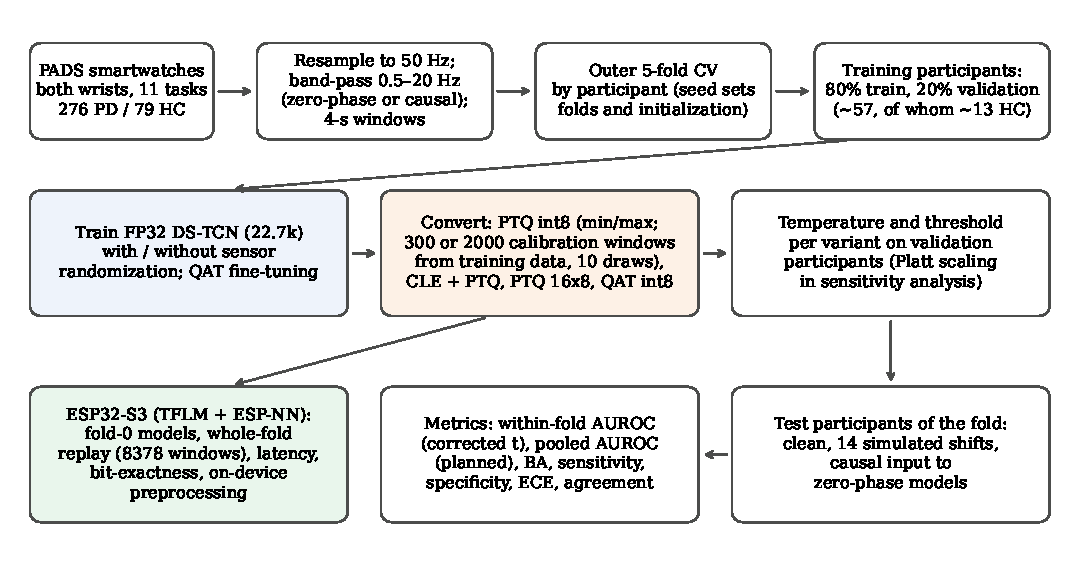
\includegraphics[width=0.85\textwidth]{Figure_1.pdf}
\caption{Study pipeline. One DS-TCN architecture is trained in six variants (FP32, PTQ and QAT, each with and without sensor randomization) in every outer fold, evaluated on PADS under 14 simulated shifts and on Monipar, and deployed on the microcontroller.}
\label{fig:pipeline}
\end{figure}

\subsection{Quantization and sensor randomization}
Networks are trained on windows with class-weighted binary cross\-entropy, Adam (learning rate $10^{-3}$, batch 512) and up to 30 epochs. Early stopping (patience 6) monitors the window AUROC on the validation participants. Six variants are built in each fold. FP32 is the full-precision model. PTQ converts it to a full-integer eight-bit model (int8 input and output) with TensorFlow Lite, calibrated on 300 training windows. QAT inserts fake-quantization nodes with the TensorFlow Model Optimization Toolkit and fine-tunes the FP32 weights for up to 5 epochs (learning rate $10^{-4}$, patience 3) before conversion. The ``+SR'' variants apply the same steps to a model trained with sensor randomization: for each training batch, a random rotation of both sensors, a gain of 0.9 to 1.1, additive noise and, with probability 0.25, the reflection that maps one wrist to the other. Every variant gets its own temperature and threshold on clean validation data; these are kept fixed under shift.

\subsection{Device-shift simulation}
Shifts are applied to the raw 100-Hz test signals before the full preprocessing chain. Sampling shifts are resampling to 50 or 25~Hz and timing jitter with a standard deviation of 10\% or 30\% of the sampling period. A different accelerometer is simulated by adding gravity in a random direction, clipping to $\pm4$~g or $\pm2$~g, quantizing to 12, 10 or 8 bits and removing gravity again. Noise shifts add white noise of 0.005 or 0.02~g and rad/s. Wearing shifts rotate both sensors by 15\textdegree, 45\textdegree\ or 180\textdegree\ about a random axis, or reflect them to emulate the other wrist. The last shift removes the gyroscope. The 50-Hz condition is identical to clean data because the pipeline already resamples to 50~Hz; it is kept as a negative control.

\subsection{Metrics and statistical analysis}
We report participant-level balanced accuracy (BA) and area under the receiver operating characteristic curve (AUROC). Confidence intervals (CIs) come from 2000 participant-level bootstrap resamples stratified by class; each participant keeps the threshold of the fold that tested it. Calibration is measured by expected calibration error (ECE, 10 bins). Agreement is the fraction of identical decisions between an eight-bit model and its full-precision parent.

The quantization analysis followed a plan fixed in a dated document before any result was seen. It has three primary hypotheses on PD versus HC with the raw input. H1: post-training quantization is non-inferior to full precision on clean data, with a margin of $-0.02$ AUROC. H2: quantization increases the mean AUROC loss over the 14 shifts. H3: quantization-aware training with sensor randomization gives a higher mean AUROC over the 14 shifts than post-training quantization. AUROC is computed on participant predictions pooled over the five outer folds. Differences use paired bootstrap resamples, and the three $p$ values are Holm-adjusted within each seed~\cite{Holm1979}. For H1, $p$ is one-sided against the margin (the bootstrap fraction of differences at or below $-0.02$); for H2 and H3, it is two-sided against zero. A hypothesis is supported only if its CI excludes the null and its adjusted $p<0.05$. Deviations are listed in Section~\ref{sec:dev}.

Pooling predictions across folds mixes five temperature-scaled models whose probability scales differ. We therefore also report, as an exploratory analysis not in the plan, the AUROC computed within each outer fold, averaged over the 15 fold--seed units of the three planned seeds. CIs use the corrected resampled $t$ statistic, which inflates the variance for overlapping training sets~\cite{Nadeau2003}. Differences inside $\pm0.02$ AUROC, the planned margin, are tested with two one-sided tests. After the first analysis, we ran exploratory experiments. With seeds 0--2, we trained and tested with the causal filter that the device uses and added three post-training variants: 2000 instead of 300 calibration windows; a full-precision model fine-tuned with the schedule of quantization-aware training but without fake quantization, then quantized; and quantization with int8 weights and int16 activations ($16\times8$). With seed 0, we also repeated the zero-phase study with a plain convolutional network without depthwise layers (41k parameters) and for PD versus DD.

\subsection{On-device deployment}
\label{sec:device}
Models are deployed on an ESP32-S3 module (dual-core Xtensa LX7 at 240~MHz, 16~MB flash, 8~MB octal PSRAM) with ESP-IDF v5.3.2, TensorFlow Lite for Microcontrollers and the ESP-NN optimized kernels. A benchmark firmware replays 50 quantized PADS test windows and compares every output byte with the reference interpreter on a desktop computer (bit-exactness). It measures network latency over 1000 invocations after 10 warm-up runs and reports the tensor-arena size actually used and the application flash footprint, with ESP-NN and with the portable reference kernels. Two further firmwares run the whole preprocessing chain on the device, per window and as a stream, and another deploys the random forest with emlearn~\cite{emlearn}.

% =====================================================================
\section{Results}
\label{sec:results}
\subsection{Participant-level benchmark (RQ1)}
Table~\ref{tab:main} lists the results. For PD versus HC, the random forest reached a BA of 0.827 and an AUROC of 0.906. The DS-TCN reached an AUROC of 0.856 (95\% CI 0.807 to 0.901) with 22.7k parameters. For PD versus DD, all networks stayed below the feature models (AUROC 0.635 to 0.685 versus 0.747). Leakage mattered: with a random window-level split, the window AUROC rose from 0.748 to 0.862 for PD versus HC and from 0.639 to 0.827 for PD versus DD. Age and sex alone gave an AUROC of 0.674 for PD versus HC, because the HC group had more women (63\% versus 29\%); the random forest AUROC stayed between 0.877 and 0.914 within each sex. Attention-based multiple-instance pooling did not improve on mean pooling, so the deployed model uses mean pooling.

\begin{table}[!t]
\caption{Participant-level results under nested cross-validation (95\% CI).}
\label{tab:main}
\centering
\resizebox{\textwidth}{!}{%
\begin{tabular}{@{}lccccc@{}}
\toprule
\multirow{2}{*}{Model} & \multirow{2}{*}{Params (k)} & \multicolumn{2}{c}{PD vs HC} & \multicolumn{2}{c}{PD vs DD} \\
\cmidrule(lr){3-4}\cmidrule(lr){5-6}
 & & BA & AUROC & BA & AUROC \\
\midrule
RF, features$^{a}$ & -- & 0.827 (0.768--0.869) & 0.906 (0.860--0.937) & 0.671 (0.603--0.710) & 0.747 (0.706--0.808) \\
XGBoost, features$^{a}$ & -- & 0.811 (0.753--0.854) & 0.907 (0.882--0.945) & 0.640 (0.601--0.705) & 0.723 (0.667--0.781) \\
DS-CNN & 11.1 & 0.739 (0.685--0.792) & 0.825 (0.772--0.873) & 0.622 (0.568--0.673) & 0.685 (0.627--0.741) \\
1-D CNN & 32.2 & 0.762 (0.712--0.809) & 0.833 (0.783--0.876) & 0.631 (0.579--0.683) & 0.661 (0.600--0.723) \\
CNN-LSTM & 44.6 & 0.755 (0.707--0.803) & 0.839 (0.790--0.883) & 0.624 (0.573--0.677) & 0.652 (0.592--0.714) \\
DS-TCN, raw & 22.7 & 0.775 (0.724--0.821) & 0.856 (0.807--0.901) & 0.601 (0.548--0.653) & 0.635 (0.573--0.695) \\
DS-TCN, invariant (Eq.~\ref{eq:inv}) & 22.7 & 0.767 (0.711--0.821) & 0.807 (0.756--0.856) & 0.609 (0.556--0.663) & 0.633 (0.573--0.693) \\
DS-TCN, raw, attention MIL & -- & 0.725 (0.669--0.776) & 0.846 (0.796--0.889) & 0.522 (0.469--0.575) & 0.551 (0.487--0.612) \\
\bottomrule
\end{tabular}}

\vspace{2pt}\parbox{\linewidth}{\footnotesize $^{a}$Point estimate: mean of three seeds; CI: seed 0. Networks: one seed, mean pooling unless noted. MIL: multiple-instance learning.}
\end{table}

\subsection{Pre-specified quantization hypotheses (RQ2, RQ3)}
Table~\ref{tab:hyp} gives the pre-specified tests on pooled predictions. Post-training quantization lowered the pooled AUROC in all three seeds ($-0.063$, $-0.064$ and $-0.033$), so non-inferiority (H1) was not shown in any seed. Quantization did not add a measurable loss under shift (H2). H3 was supported in seeds 0 and 2 but not in seed 1.

\begin{table}[!t]
\caption{Pre-specified hypotheses on pooled predictions (PD versus HC, raw input).}
\label{tab:hyp}
\centering\small
\begin{tabular}{@{}llccc@{}}
\toprule
Hypothesis & Seed & Estimate (95\% CI) & $p_\text{Holm}$ & Supported \\
\midrule
H1 & 0 & $-0.063$ ($-0.115$, $-0.013$) & 0.95 & No \\
 & 1 & $-0.064$ ($-0.103$, $-0.027$) & 1.00 & No \\
 & 2 & $-0.033$ ($-0.100$, $+0.035$) & 1.00 & No \\
H2 & 0 & $+0.008$ ($-0.007$, $+0.023$) & 0.61 & No \\
 & 1 & $-0.002$ ($-0.013$, $+0.008$) & 1.00 & No \\
 & 2 & $-0.000$ ($-0.013$, $+0.012$) & 1.00 & No \\
H3 & 0 & $+0.133$ ($+0.062$, $+0.207$) & 0.0015 & Yes \\
 & 1 & $+0.045$ ($-0.005$, $+0.093$) & 0.25 & No \\
 & 2 & $+0.122$ ($+0.054$, $+0.195$) & 0.003 & Yes \\
\bottomrule
\end{tabular}

\vspace{2pt}\parbox{\linewidth}{\footnotesize H1: PTQ$-$FP32, clean, one-sided against margin $-0.02$. H2: loss of PTQ minus loss of FP32 (clean minus 14-shift mean). H3: QAT+SR$-$PTQ, 14-shift mean. Seed 0 is primary; Holm correction within each seed.}
\end{table}

\subsection{Within-fold analysis (exploratory)}
The pooled AUROC of the full-precision model (0.762 in seed 0) was much lower than its within-fold AUROC (0.879); the pooled benchmark of Table~\ref{tab:main} (0.856) came from a different implementation and training run. Within each fold, the model ranks participants well, but the five folds place their probabilities on different scales after temperature scaling, so the pooled tests mix ranking and calibration. Table~\ref{tab:quant} and Fig.~\ref{fig:shift} report the within-fold AUROC over the 15 fold--seed units. Post-training quantization lost 0.066 (95\% CI 0.001 to 0.130); 13 of 15 units lost more than 0.02, and one lost 0.219. Quantization-aware training differed from full precision by $+0.003$ ($-0.027$ to $0.033$); equivalence within $\pm0.02$ was not established ($p=0.12$). On the shift mean, it beat post-training quantization by 0.068 (0.008 to 0.128). The H3 contrast was $+0.038$ ($-0.054$ to $0.130$). Sensor randomization changed the clean AUROC by $-0.027$ ($-0.085$ to $0.031$) and the shift mean of quantization-aware training by $-0.030$ ($-0.079$ to $0.019$). It helped for a 180\textdegree\ rotation (FP32 + SR 0.837 versus FP32 0.772). After sensor randomization, post-training quantization lost only 0.007 ($-0.044$ to $0.030$). All variants lost accuracy without the gyroscope. As H2 indicated, quantization losses were present on clean data and did not grow under shift.

\begin{table}[!t]
\caption{Training variants for PD versus HC (raw input, zero-phase filter, within-fold AUROC, 15 fold--seed units).}
\label{tab:quant}
\centering\small
\begin{tabular}{@{}lccccc@{}}
\toprule
 & \multicolumn{2}{c}{AUROC} & \multicolumn{3}{c}{Clean} \\
\cmidrule(lr){2-3}\cmidrule(lr){4-6}
Variant & Clean & Shift mean & BA & ECE & Agreement \\
\midrule
FP32 & 0.874 & 0.860 & 0.769 & 0.126 & 1.000 \\
PTQ INT8 & 0.808 & 0.794 & 0.703 & 0.114 & 0.818 \\
QAT INT8 & 0.877 & 0.861 & 0.797 & 0.121 & 0.856 \\
FP32 + SR & 0.847 & 0.842 & 0.746 & 0.119 & 1.000 \\
PTQ INT8 + SR & 0.840 & 0.833 & 0.744 & 0.133 & 0.845 \\
QAT INT8 + SR & 0.840 & 0.832 & 0.737 & 0.121 & 0.865 \\
\bottomrule
\end{tabular}

\vspace{2pt}\parbox{\linewidth}{\footnotesize Means over seeds 0--2. Shift mean: 14 pre-specified shifts. Agreement: decisions identical to the full-precision parent. SR: sensor randomization.}
\end{table}

\begin{figure}[!t]
\centering
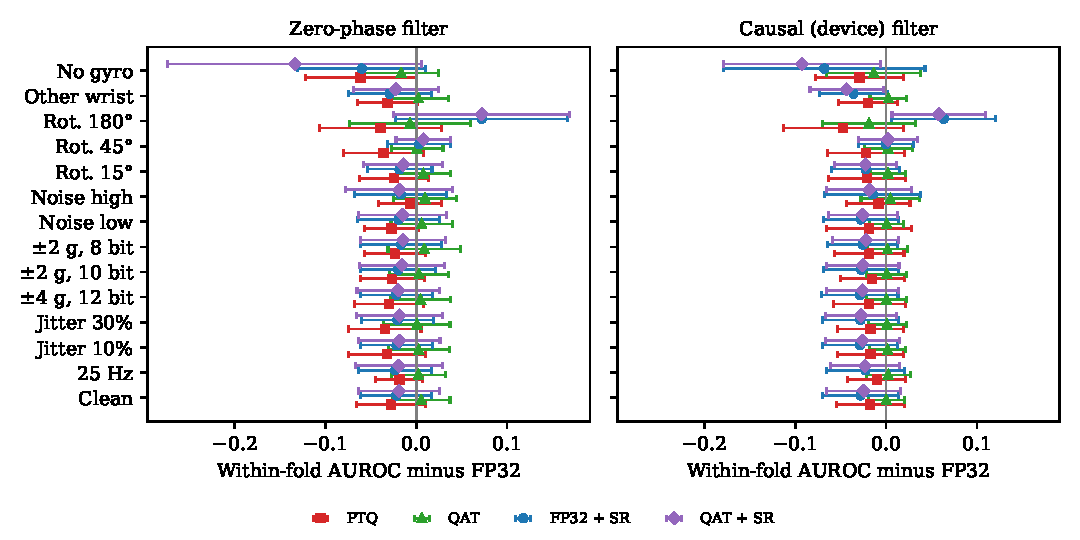
\includegraphics[width=0.85\textwidth]{Figure_2.pdf}
\caption{Within-fold AUROC for PD versus HC under each simulated shift (mean and 95\% CI over 15 fold--seed units). The 50-Hz condition equals the clean condition and is not shown.}
\label{fig:shift}
\end{figure}

\subsection{Device-matched and further exploratory runs}
Table~\ref{tab:explore} lists the three-seed runs with the device's causal filter. Full precision reached a within-fold AUROC of 0.866. Post-training quantization lost 0.025 on average ($-0.074$ to $0.024$), with 8 of 15 units losing more than 0.02 and one losing 0.119. More calibration windows (loss 0.017) and fine-tuning before quantization (loss 0.020 relative to the fine-tuned model) did not remove the instability. Keeping activations at 16 bits did: the $16\times8$ model differed from full precision by $-0.001$ ($-0.004$ to $0.001$), was equivalent within $\pm0.02$ ($p<0.001$), and lost at most 0.005 in any unit. The loss of post-training quantization therefore comes from 8-bit activations, not from 8-bit weights. Quantization-aware training was equivalent to the fine-tuned full-precision model ($+0.004$, $-0.011$ to $0.018$; $p=0.016$). Sensor randomization again lowered the clean AUROC ($-0.039$), and the H3 contrast was $-0.009$.

In seed-0 runs with zero-phase filtering, post-training quantization of a plain convolutional network lost nothing ($-0.001$), and quantization-aware training was at least as good as full precision. For PD versus DD, full precision reached 0.689; post-training quantization lost 0.040 on average and 0.126 in one fold, quantization-aware training stayed within 0.006 of full precision, and the H3 contrast was $+0.002$.

\begin{table}[!t]
\caption{Exploratory runs with the device's causal filter (PD versus HC, within-fold AUROC, 15 fold--seed units).}
\label{tab:explore}
\centering\small
\begin{tabular}{@{}lccc@{}}
\toprule
Variant & Clean & Shift mean & Clean $-$ reference (95\% CI) \\
\midrule
FP32 (reference) & 0.866 & 0.853 & -- \\
PTQ, 300 windows & 0.841 & 0.828 & $-0.025$ ($-0.074$, $0.024$) \\
PTQ, 2000 windows & 0.849 & 0.832 & $-0.017$ ($-0.053$, $0.019$) \\
PTQ $16\times8$ & 0.865 & 0.852 & $-0.001$ ($-0.004$, $0.001$) \\
FP32 fine-tuned$^{a}$ & 0.881 & 0.867 & $+0.015$ ($-0.016$, $0.045$) \\
PTQ of fine-tuned$^{a}$ & 0.860 & 0.843 & $-0.020$ ($-0.055$, $0.015$) \\
QAT & 0.884 & 0.866 & $+0.019$ ($-0.010$, $0.047$) \\
QAT + SR & 0.827 & 0.819 & $-0.039$ ($-0.097$, $0.019$) \\
\bottomrule
\end{tabular}

\vspace{2pt}\parbox{\linewidth}{\footnotesize $^{a}$Same schedule as QAT, no fake quantization; PTQ of fine-tuned is compared with the fine-tuned model. $16\times8$: int8 weights, int16 activations. CIs: corrected resampled $t$.}
\end{table}

\subsection{External cohort (descriptive)}
For Monipar, each variant was trained once on 80\% of the PADS participants with PD or HC, using the three matched tasks and acceleration only, with temperature and threshold fitted on the remaining 20\%. The models were then tested on Monipar without any adaptation. The 0.5-Hz high-pass edge of the band-pass filter removes gravity from the Monipar signals, which matches the gravity-free PADS acceleration. Table~\ref{tab:monipar} lists the results. With the acceleration input, the FP32 model reached an AUROC of 0.857 (95\% CI 0.701 to 0.980); the eight-bit variants ranged from 0.490 to 0.946. With two invariant acceleration channels, they ranged from 0.524 to 0.837. The CIs spanned 0.3 to 0.4 AUROC units, and the ranking of variants was not consistent across the two inputs. Some models gave nearly the same probability to every participant, so the PADS threshold did not transfer. We therefore draw no conclusion about quantization from this cohort.

\begin{table}[!t]
\caption{Zero-shot results on Monipar (21 PD, 7 HC).}
\label{tab:monipar}
\centering\small
\begin{tabular}{@{}lcccc@{}}
\toprule
 & \multicolumn{2}{c}{Acceleration (4 channels)} & \multicolumn{2}{c}{Invariant (2 channels)} \\
\cmidrule(lr){2-3}\cmidrule(lr){4-5}
Variant & AUROC (95\% CI) & BA & AUROC (95\% CI) & BA \\
\midrule
FP32 & 0.857 (0.70--0.98) & 0.833 & 0.728 (0.51--0.89) & 0.643 \\
PTQ & 0.946 (0.83--1.00) & 0.714 & 0.524 (0.29--0.75) & 0.476 \\
QAT & 0.864 (0.71--0.99) & 0.810 & 0.782 (0.58--0.94) & 0.619 \\
FP32 + SR & 0.796 (0.59--0.96) & 0.714 & 0.769 (0.58--0.92) & 0.476 \\
PTQ + SR & 0.490 (0.28--0.70) & 0.500 & 0.837 (0.67--0.97) & 0.762 \\
QAT + SR & 0.707 (0.49--0.89) & 0.595 & 0.701 (0.50--0.88) & 0.667 \\
\bottomrule
\end{tabular}

\vspace{2pt}\parbox{\linewidth}{\footnotesize Acceleration: $\mathbf{a}$ and $\|\mathbf{a}\|$. Invariant: $\|\mathbf{a}\|$ and $\|\Delta\mathbf{a}\|$. One training run.}
\end{table}

\subsection{On-device measurements}
Table~\ref{tab:board} lists the fold-0 models on the ESP32-S3. All 50 replayed windows gave outputs identical to the reference interpreter (maximum difference 0 least significant bits). With ESP-NN, one 4-s window took 11.6~ms, or 0.3\% of real time; the portable kernels were 6.1 times slower. QAT and QAT + SR models had the same latency and arena as the PTQ model, and the model file grew by 1.4~kB (49.5 to 50.9~kB).

A second firmware ran the whole pipeline on the device from raw 100-Hz samples: polyphase decimation to 50~Hz, a causal fourth-order Butterworth band-pass filter, channel construction, normalization, quantization and inference. One 4-s window took 14.6~ms end to end (p95 14.7~ms), of which preprocessing took 2.4~ms, with 42.6~kB of RAM and a 472-kB application image. Its outputs matched a causal Python implementation bit for bit on eight windows. The model trained with zero-phase filtering, however, changed its predicted probability by up to 0.28 on these windows when fed causally filtered signals. On the 71 fold-0 test participants, its AUROC fell from 0.890 to 0.816 and 18\% of its decisions changed. A third firmware therefore ran the causally trained QAT model on whole PADS recordings as a stream. It decimated and filtered each 2-s block with persistent filter states and classified a 4-s window every 2~s. Each step took 12.6~ms (p95 12.7~ms): 1.0~ms for preprocessing and 11.6~ms for normalization, quantization and inference. Outputs were bit-exact with the causal Python pipeline for 27 of 27 windows from three recordings, and the pipeline used 39.4~kB of RAM.

A USB power meter with 10-mA resolution showed about 70~mA at 5.1~V for the whole board during continuous inference. In a 4-s duty cycle with light sleep, the processor was active for 0.4\% of the time, and the current stayed below the meter's resolution; we do not derive energy per window from these coarse readings.

We also deployed the feature-based random forest (fold 0; 100 trees, depth 8; 2112 features from 22 task--wrist recordings). Its fold-0 test AUROC was 0.923. On the device, the forest took 2.5~ms per participant and agreed with scikit-learn on 20 of 20 test participants. Computing the 96 features of one 10-s recording, including a causal filter and Welch spectra, took 10.5~ms, and the features matched Python within a relative error of $3\times10^{-4}$. A full 22-recording assessment would therefore take about 0.23~s on the device. The forest needs no quantization, but it requires the complete two-wrist, eleven-task protocol, whereas the network scores any 4-s window from one wrist.

\begin{table}[!t]
\caption{Network inference on the ESP32-S3 (240 MHz, fold-0 models).}
\label{tab:board}
\centering\small
\begin{tabular}{@{}llcccc@{}}
\toprule
Model & Kernels & Latency (ms) & Arena (kB) & Image (kB) & Bit-exact \\
\midrule
PTQ & ESP-NN & 11.56 & 21.2 & 448 & 50/50 \\
PTQ & Portable & 70.29 & 20.2 & 414 & 50/50 \\
QAT & ESP-NN & 11.54 & 21.2 & 449 & 50/50 \\
QAT & Portable & 70.32 & 20.2 & 415 & 50/50 \\
QAT + SR & ESP-NN & 11.56 & 21.2 & 449 & 50/50 \\
QAT + SR & Portable & 70.32 & 20.2 & 415 & 50/50 \\
\bottomrule
\end{tabular}

\vspace{2pt}\parbox{\linewidth}{\footnotesize Latency: mean of 1000 runs (p95 within 0.15 ms). Image: application firmware image.}
\end{table}

% =====================================================================
\section{Discussion}
\label{sec:discussion}
This study asked whether a microcontroller-sized network for Parkinson's disease detection keeps its accuracy after eight-bit quantization. For the depthwise-separable network, post-training quantization did not. The pre-specified non-inferiority test failed in every seed. Within folds, the loss averaged 0.066 AUROC, varied strongly between folds and runs, and reached 0.219 in one fold. In the causal runs, a larger calibration set did not remove it. Quantization-aware training showed no detectable loss, stayed close to a full-precision model fine-tuned on the same schedule, and had the same latency, memory and bit-exactness on the device. For a plain convolutional network, post-training quantization was harmless. The $16\times8$ experiment located the problem: with 16-bit activations and 8-bit weights, the loss vanished in every unit. Activation ranges in depthwise convolutions differ widely between channels, which per-tensor activation quantization handles poorly~\cite{Krishnamoorthi2018,Nagel2021}. A single successful post-training conversion is therefore weak evidence that a quantized model is safe.

The pre-specified method, quantization-aware training with sensor randomization, beat post-training quantization on pooled predictions in two of three seeds. This is the primary result. Within folds, its advantage was smaller and not significant, and sensor randomization gave no consistent benefit except for large rotations, which correspond to a watch worn upside down. Most of the pooled advantage therefore seems to come from avoiding the post-training loss rather than from robustness to shift. Because the within-fold analysis was not planned, we present these readings as exploratory. They agree with H2: quantization did not interact with shift.

The gap between pooled and within-fold AUROC is a methodological lesson in itself. Temperature scaling on a small validation set gives each fold its own probability scale, and pooling such predictions lowered the AUROC by more than 0.1 and could create or hide differences between variants. Calibration is also model-specific after quantization: in embedded electrocardiogram classification, reusing the full-precision calibration on the INT8 model broke conformal coverage until it was refitted on INT8 outputs~\cite{ElAllam2026}. We fitted temperature and threshold separately for every variant for the same reason. Studies that pool cross-validated predictions should check within-fold metrics as well.

On-device validation exposed a mismatch that desktop evaluation hides. Zero-phase filtering cannot run in real time, and a model trained with it lost 0.074 AUROC when fed causally filtered signals. Training with the causal filter that the device uses removed this loss. Bit-exact kernels are necessary but not sufficient; the whole preprocessing chain must match. The same concern applies across devices, because filtering choices also determine how equivalent the raw signals of different accelerometers are~\cite{CoyleAsbil2026}.

The benchmark puts the networks in context. On PADS, hand-crafted features with a random forest reached a higher AUROC than every network, especially for PD versus other movement disorders, and the forest also ran on the microcontroller. Small networks remain attractive because they score a single window from one wrist, but they are not yet more accurate than features on this cohort. Window-level splitting would have hidden this gap: it raised the window AUROC by 0.11 to 0.19~\cite{Saeb2017,Kapoor2023}. The external cohort did not settle the question of real device shift. With seven controls, the CIs spanned 0.3 to 0.4 AUROC units, the ranking of variants changed with the input, and a threshold learned on PADS did not transfer; small wearable cohorts in PD give similarly wide estimates~\cite{Magni2026}. A larger independent cohort recorded with a different watch is needed.

\subsection{Deviations from the analysis plan}
\label{sec:dev}
The executed network placed the stride of blocks two and four in the depthwise convolution, whereas the frozen script placed it in the pointwise convolution; the parameter count is the same. The 50-Hz shift equals the clean condition but was kept, as planned; removing it does not change H3 (within-fold difference 0.038 in both cases for seeds 0--2). The Monipar run initially failed for technical reasons and was repeated with an equivalent stride setting. The within-fold analysis and the exploratory runs were added after the first results.

\subsection{Limitations}
The shifts were simulated; they approximate, but do not reproduce, a different device. The external cohort is small and has no gyroscope. The plain-network and PD-versus-DD runs use one seed, and a repeated run showed that training is not fully deterministic. Cross-layer equalization, bias correction and adaptive rounding were not tested, and the $16\times8$ model was not run on the device. Age and sex were unbalanced between PD and HC; the feature model kept its accuracy within each sex, but we did not stratify the network results. The data come from a clinic, so the results concern detection in a referred population rather than population screening. The deployed random forest was trained on features from zero-phase filtering, while the device computed them with a causal filter; its on-device accuracy was not re-estimated. The streaming pipeline was checked on three recordings. The pre-specified experiments used zero-phase filtering, which cannot run on the device, and energy was measured only with a coarse USB meter. Finally, only one microcontroller family and two architectures were tested.

% =====================================================================
\section{Conclusions}
\label{sec:conclusion}
In a pre-specified three-seed study, post-training eight-bit quantization of a tiny depthwise-separable network for Parkinson's disease detection was not non-inferior to full precision, and its loss varied strongly between folds. The combined method with quantization-aware training beat it in two of three seeds. Exploratory analyses traced the post-training loss to 8-bit activations and attributed the gain to quantization-aware training rather than to sensor randomization. Quantization-aware training added no latency or working memory on an ESP32-S3 microcontroller, where bit-exact streaming inference required a network trained with the device's own causal filter. Quantized wearable models should be validated per fold, across seeds and with the device's preprocessing.

% =====================================================================
\section*{CRediT authorship contribution statement}
\textbf{Quang-Tuyen Lai:} Conceptualization, Methodology, Software, Investigation, Formal analysis, Data curation, Visualization, Writing -- original draft. \textbf{Ba-Viet Ngo:} Conceptualization, Methodology, Supervision, Validation, Writing -- review \& editing.

\section*{Declaration of competing interest}
The authors declare that they have no known competing financial interests or personal relationships that could have appeared to influence the work reported in this paper.

\section*{Funding}
This research did not receive any specific grant from funding agencies in the public, commercial, or not-for-profit sectors.

\section*{Ethics statement}
This study used only two publicly available, de-identified datasets~\cite{PADSdata,MoniparData}. No new data were collected from human participants, so no additional ethical approval was required.

\section*{Data availability}
PADS~\cite{PADSdata} and Monipar~\cite{MoniparData} are publicly available. The code is available from the corresponding author on reasonable request.

\section*{Declaration of generative AI and AI-assisted technologies in the manuscript preparation process}
During the preparation of this work the authors used Claude (Opus 5.5, Anthropic) in order to assist with writing analysis and firmware code, running the statistical analyses, and drafting and editing the manuscript. After using this tool, the authors reviewed and edited the content as needed and take full responsibility for the content of the published article.

\bibliographystyle{elsarticle-num}
\bibliography{refs}

\end{document}
